\documentclass{article}
\usepackage[a4paper,margin= 2cm]{geometry}
\usepackage{graphicx}

\title{\LARGE{\bf{Task 1 Overview}}}
\author{\Large{\bf{Kirtan Patel - AE19B038}}}
\date{}

\begin{document}

\maketitle 

\section{The Amplitude Magnification Frequency Response Graph}
This Graph shows the relation between the Amplitude Magnification Function and the Frequency of the Sytem. The Frequency $\omega$ is given as a ratio over the natural frequency of the system $\omega_{n}$.
\[x(t) = \delta_{static}~|G(i\omega)|~e^{i(\omega t - \phi)}\]
where
\[|G(i \omega)|^2 = \frac{1}{(1 - r^2)^2 + (2 \zeta r)^2}\]
\begin{figure}
\centering
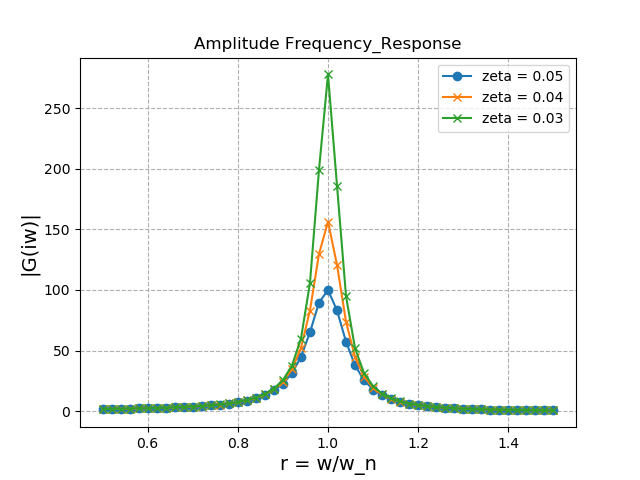
\includegraphics[scale = 0.56]{Amplitude Frequency_Response.png}
\caption{Frequency Response of Amplitude Magnification}
\label{fig1.}
\end{figure}

This Graph helps us analyse the nature of vibrations experienced by the system under study. Studying the graph, we can observe that:
\begin{enumerate}
	\item For an undamped system($\zeta$=0),and G$\rightarrow$ $\infty$ as r $\rightarrow$ 1
	\item Any amount of damping($\zeta$$>$0)reduces the magnification factor (G) for all values of the forcing frequency.
	\item In the degenerate case of a constant force (when r=0), the value of $|G|$
	\item The reduction in $|G|$ in the presence of damping is very significant at or near resonance.
\end{enumerate}

In System Design, we use this data to design the structure such that the frequency of vibrations handled by the structure are not near the natural frequency of the structure and hence limit the Magnification of the Transferred Vibrations.\\ 

The graph even helps us predict the values of Magnification Factor for intermediate Frequency Ratios by interpolation. Hence, this graph is widely used in the study and design of systems which are subjected to vibrations
\pagebreak


\section{Sinusoidal Multivariable Function Plot}
This Graph shows the sinusoidal relation expressed as
\[z(x,y) = \frac{sin(5x).cos(5y)}{5}\]

This Graph helps us analyse the nature of multivariable functions.It contains multiple Saddle Points and can be used in visualizing the concept.\\

\begin{figure} [!ht] %to keep the image where we place it.
\centering
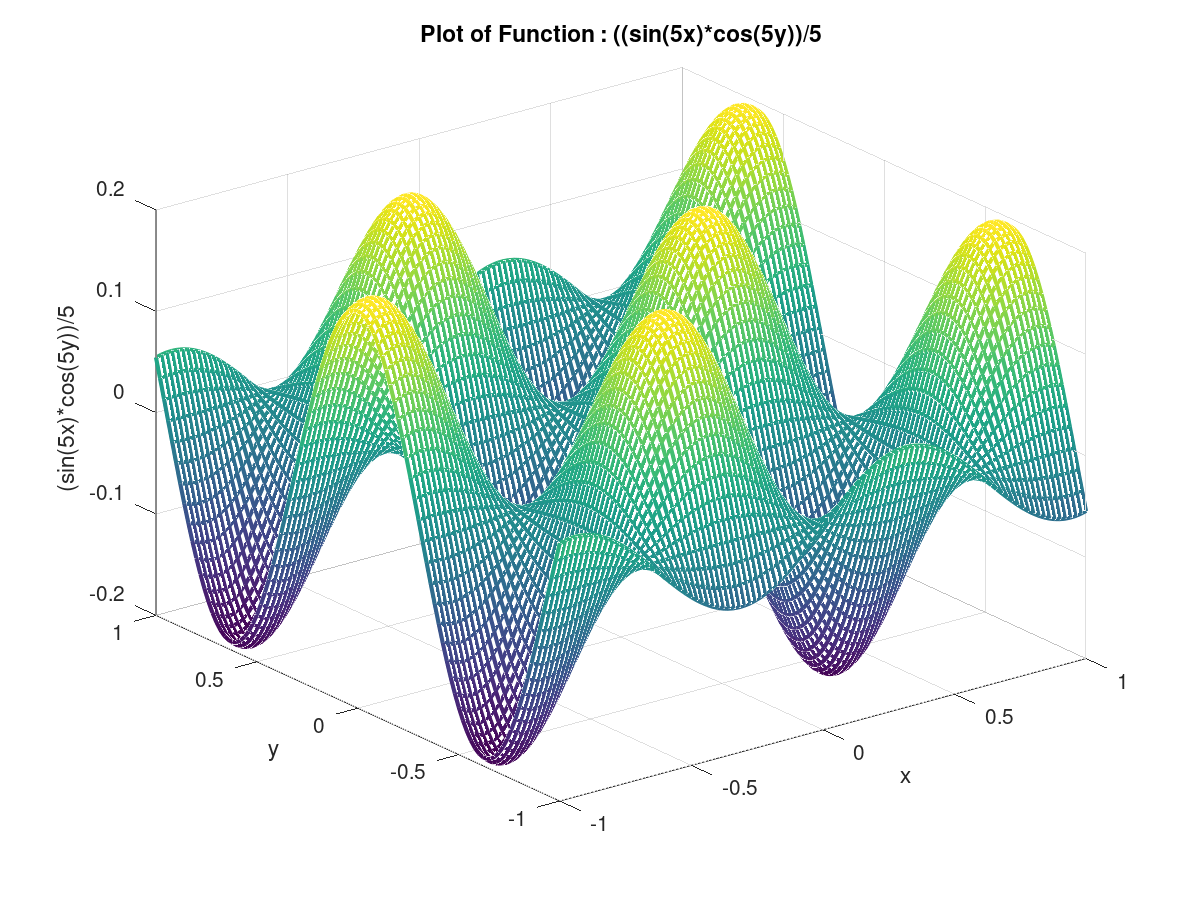
\includegraphics[scale=0.3]{Octave_3D Plot.png}
\caption{Sinusoidal Multivariable Function Plot}
\label{fig2.}
\end{figure}


\subsection{Saddle Point}
Given the function z=f(x,y), the point $(x_{0},y_{0},f(x_{0},y_{0}))$ is a saddle point if both $f_{x}(x_{0},y_{0})=0$ and $f_{y}(x_{0},y_{0})=0$, but f does not have a local extremum at $(x_{0},y_{0})$.\\

While we have to be careful to not misinterpret the results of this fact it is very useful in helping us to identify relative extrema. Because of this fact we know that if we have all the critical points of a function then we also have every possible relative extrema for the function. The fact tells us that all relative extrema must be critical points so we know that if the function does have relative extrema then they must be in the collection of all the critical points. Remember however, that it will be completely possible that at least one of the critical points won’t be a relative extrema.\\

In machine learning for example, local/global minimums/maximums are important as the indicate the validity and accuracy of the function.
\end{document}